% Sección 5: Resultados predictivos por familia de evidencia
% evidencia:E08,E09,E12,E13,E14

\section{Resultados predictivos por familia de evidencia}

Siguiendo la separación metodológica establecida en la sección anterior, los resultados predictivos se presentan en tres bloques independientes: la corrida experimental puntual de demanda del 18 de noviembre de 2026, los metadatos archivados del artefacto cuantílico servido en la web (\texttt{v2.0}) en contraste con el reporte histórico de intervalos del 3 de noviembre, y las dos corridas comprobadas para el horizonte extendido a 120 días.

\subsection{Experimento puntual Poisson: escalera, servicios, festivos y estabilidad}

En los 26 pliegues \textit{walk-forward} del experimento puntual reportado el 18 de noviembre de 2026 \parencite{mediflow2026demanda}, la incorporación progresiva de estructura estratificada por servicio, nivel local con pesos por recencia y factores externos validados reduce el error global de manera consistente. La Tabla~\ref{tab:escalera_poisson} recoge las métricas globales de la escalera sin incluir la serie residual \texttt{Otros}.

\begin{table}[htbp]
\caption{Escalera predictiva puntual en 26 pliegues \textit{walk-forward} (experimento del 18 de noviembre de 2026)}
\label{tab:escalera_poisson}
{\singlespacing\small
\begin{tabularx}{\textwidth}{@{}Y r r r r r@{}}
\toprule
Modelo evaluado & WAPE & MAE & RMSE & Sesgo & Mejora rel. \\
\midrule
1. Línea base (mediana de 8 semanas) & 18,0\,\% & 77,02 & 201,34 & $+21{,}44$ & Referencia \\
2. Poisson estratificado por servicio & 15,6\,\% & 66,86 & 125,91 & $+6{,}41$ & $+13{,}2\,\%$ \\
3. LightGBM nivel local (todos externos) & 10,5\,\% & 44,84 & 83,82 & $-6{,}00$ & $+41{,}8\,\%$ \\
4. LightGBM Poisson final (\texttt{lgbm\_final}) & 10,5\,\% & 44,94 & 83,67 & $-5{,}70$ & $+41{,}6\,\%$ \\
\bottomrule
\end{tabularx}}
\apanota{Datos archivados de \textcite{mediflow2026demanda}, sección~1 (orígenes \texttt{2025-07-25} a \texttt{2026-07-10}, horizonte 1--7 días). Las mejoras relativas frente a la línea base fueron calculadas con las cifras sin redondear antes de su publicación, por lo que no deben recalcularse a partir de 18,0\,\% y 10,5\,\% redondeados. El modelo \texttt{lgbm\_final} conserva únicamente los grupos aceptados (\texttt{festivos\_y\_puentes} y \texttt{carnaval\_y\_semana\_santa}) y se selecciona por parsimonia y respaldo empírico, aunque los dos escalones LightGBM coincidan en WAPE a una decimal.}
\end{table}

El desempeño desagregado del modelo seleccionado \texttt{lgbm\_final} evidencia una fuerte heterogeneidad entre servicios (Tabla~\ref{tab:servicios_poisson}). En Urgencias (\texttt{9203}) y Rehabilitación Ambulatoria (\texttt{581479}), el error WAPE global es de 8,4\,\% y 11,0\,\% (exactitudes $1-\text{WAPE}$ de 91,6\,\% y 89,0\,\%, respectivamente). Sin embargo, el detalle por día de la semana confirma que en Rehabilitación la exactitud cae a 51,3\,\% los sábados (media de 87,1 llegadas/día) y a 15,6\,\% los domingos (media de 2,2 llegadas/día), frente a valores de 85,6\,\% a 90,9\,\% entre lunes y viernes (835,7 a 1.306,2 llegadas/día) \parencite{mediflow2026demanda}. En Tratamiento Urgencias (\texttt{3045729}), con una media de 15,17 llegadas/día, el WAPE diario alcanza 43,5\,\% (exactitud 56,5\,\%, MAE 6,59 pacientes). Contrastado contra el techo idealizado de Poisson, el modelo alcanza 56,5\,\% diario frente a un techo de 79,5\,\%, y al agregar la semana completa en los 26 pliegues alcanza 77,0\,\% frente a un techo semanal de 92,3\,\% \parencite{mediflow2026demanda}. Dado que permanece por debajo de ambas cotas optimistas, el error de este servicio obedece tanto a la varianza de conteos bajos como a cambios semanales en su tasa subyacente, por lo que no debe declararse cumplida la meta operativa diaria.

\begin{table}[htbp]
\caption{Desempeño por servicio del experimento puntual \texttt{lgbm\_final}}
\label{tab:servicios_poisson}
{\singlespacing\small
\begin{tabularx}{\textwidth}{@{}Y r r r r r@{}}
\toprule
Servicio & WAPE & $1-\text{WAPE}$ & MAE & Sesgo & Prom. real \\
\midrule
Emergency Room Visit (\texttt{9203}) & 8,4\,\% & 91,6\,\% & 37,02 & $-7{,}83$ & 443,16 \\
Ambulatory Rehab. (\texttt{581479}) & 11,0\,\% & 89,0\,\% & 91,22 & $-10{,}12$ & 826,54 \\
Treatment urgency (\texttt{3045729}) & 43,5\,\% & 56,5\,\% & 6,59 & $+0{,}86$ & 15,17 \\
\bottomrule
\end{tabularx}}
\apanota{Datos archivados de \textcite{mediflow2026demanda}, sección~2 (26 pliegues, 182 días por servicio, excluyendo \texttt{Otros}). Estas métricas pertenecen al experimento LightGBM Poisson y no deben transferirse al modelo cuantílico servido en la aplicación web.}
\end{table}

Al comparar días normales frente a días festivos \parencite{mediflow2026demanda}, en días normales el WAPE desciende de 12,4\,\% en la línea base (MAE 55,63; sesgo $-3{,}45$) a 10,3\,\% en \texttt{lgbm\_final} (MAE 45,97; sesgo $-6{,}96$), mientras que en días festivos la línea base exhibe WAPE de 317,8\,\% (MAE 409,64; sesgo $+408{,}36$) debido a la sobreestimación masiva cuando Rehabilitación cierra casi por completo, frente a 22,5\,\% en \texttt{lgbm\_final} (MAE 29,03; sesgo $+13{,}89$). Este contraste refleja el efecto mecánico de dividir por un volumen festivo muy bajo en la métrica base y la captura calendárica del modelo, no un impacto causal sobre la demanda hospitalaria. A lo largo del horizonte 1--7 días, el WAPE agregado oscila entre 9,4\,\% (día 7, jueves) y 17,0\,\% (día 2, sábado); entre pliegues individuales, oscila entre 5,4\,\% (pliegue 17, \texttt{2026-03-20}) y 28,0\,\% en el pliegue 11 (\texttt{2025-12-26}, fin de año, donde la línea base alcanza 137,9\,\%) y 27,6\,\% en el pliegue 19 (\texttt{2026-04-17}) \parencite{mediflow2026demanda}. Las series completas de los 26 pliegues y la matriz por servicio y día se conservan en el Anexo~B.

\subsection{Artefacto cuantílico servido en la aplicación web (\texttt{v2.0})}

Los metadatos efectivamente empaquetados en \texttt{models/modelos\_web\_bundle.joblib} (inspeccionados directamente sin reejecutar entrenamientos ni consultas a base de datos) muestran el rendimiento fuera de muestra sobre 182 días (\texttt{2025-07-25} a \texttt{2026-07-16}) de la variante cuantílica $p_{10}/p_{50}/p_{90}$ consumida por la API web. La Tabla~\ref{tab:bundle_cuantilico} expone sus métricas separadas de la Tabla~\ref{tab:servicios_poisson}. En Urgencias el WAPE de $p_{50}$ es 8,91\,\% (frente a 8,4\,\% del experimento Poisson), en Rehabilitación 11,08\,\% y en Tratamiento Urgencias 42,18\,\%. La cobertura empírica $p_{10}$--$p_{90}$ almacenada asciende a 78,57\,\% en Urgencias, 64,29\,\% en Rehabilitación y 73,08\,\% en Tratamiento Urgencias, quedando por debajo del objetivo nominal de 80\,\%, especialmente en Rehabilitación donde los cierres bruscos y la ausencia de nivel local multiplicativo estrechan o desalinean las bandas.

\begin{table}[htbp]
\caption{Métricas archivadas del modelo cuantílico servido en el artefacto web \texttt{v2.0}}
\label{tab:bundle_cuantilico}
{\singlespacing\small
\begin{tabularx}{\textwidth}{@{}Y r r r r r r@{}}
\toprule
Servicio en bundle \texttt{v2.0} & WAPE & MAE & RMSE & Sesgo & Cob. $p_{10}$--$p_{90}$ & Exact. sem. \\
\midrule
Urgencias (\texttt{9203}) & 8,91\,\% & 39,50 & 53,82 & $-2{,}69$ & 78,57\,\% & 94,75\,\% \\
Rehabilitación (\texttt{581479}) & 11,08\,\% & 91,55 & 137,57 & $+4{,}22$ & 64,29\,\% & 91,63\,\% \\
Tratamiento Urg. (\texttt{3045729}) & 42,18\,\% & 6,40 & 8,47 & $-0{,}64$ & 73,08\,\% & 76,60\,\% \\
\bottomrule
\end{tabularx}}
\apanota{Metadatos almacenados en \texttt{comparacion\_real} de \texttt{models/modelos\_web\_bundle.joblib} \parencite{mediflow2026bundle} sobre 182 días (\texttt{2025-07-25} a \texttt{2026-07-16}, corte exclusivo \texttt{2026-07-17}), consultables también vía \texttt{GET /api/modelo}. Las métricas de cobertura fueron calculadas antes de redondear los puntos servidos a enteros; recomputar sobre salidas enteras puede modificar ligeramente la cobertura observada. Techos Poisson almacenados: Urgencias 96,21\,\% diario / 98,57\,\% semanal; Rehabilitación 97,22\,\% / 98,95\,\%; Tratamiento Urgencias 79,53\,\% / 92,26\,\%.}
\end{table}

Resulta indispensable distinguir estas cifras de la corrida histórica archivada en \textcite{mediflow2026intervalos} del 3 de noviembre de 2026. En aquel reporte anterior se documentó una cobertura global de 83,2\,\% (85,2\,\% en Urgencias, 72,0\,\% en Rehabilitación, 75,8\,\% en Tratamiento Urgencias y 100,0\,\% en \texttt{Otros}, con amplitud media de 112,6 pacientes). Al incluir la categoría \texttt{Otros} (donde la cobertura alcanza 100\,\% por volumen casi nulo) y pertenecer a una versión anterior previa a la actualización del 18--19 de noviembre, esa cifra de 83,2\,\% no valida ni representa la calibración del bundle \texttt{v2.0} actual. Adicionalmente, cuando la aplicación web consulta fechas futuras o sin rezagos observados, \texttt{predict.py} sustituye los rezagos faltantes por medianas históricas de día de la semana (\texttt{medianas\_dw}), comportamiento que no hereda la validación de 1--7 días.

La Figura~\ref{fig:resumen_escalera} resume visualmente la distancia metodológica entre la escalera predictiva puntual de esta sección y la simulación histórica de altas tempranas abordada en optimización.

\begin{figure}[htbp]
\caption{Síntesis comparativa entre evaluación predictiva puntual y simulación histórica de altas}
\label{fig:resumen_escalera}
\centering
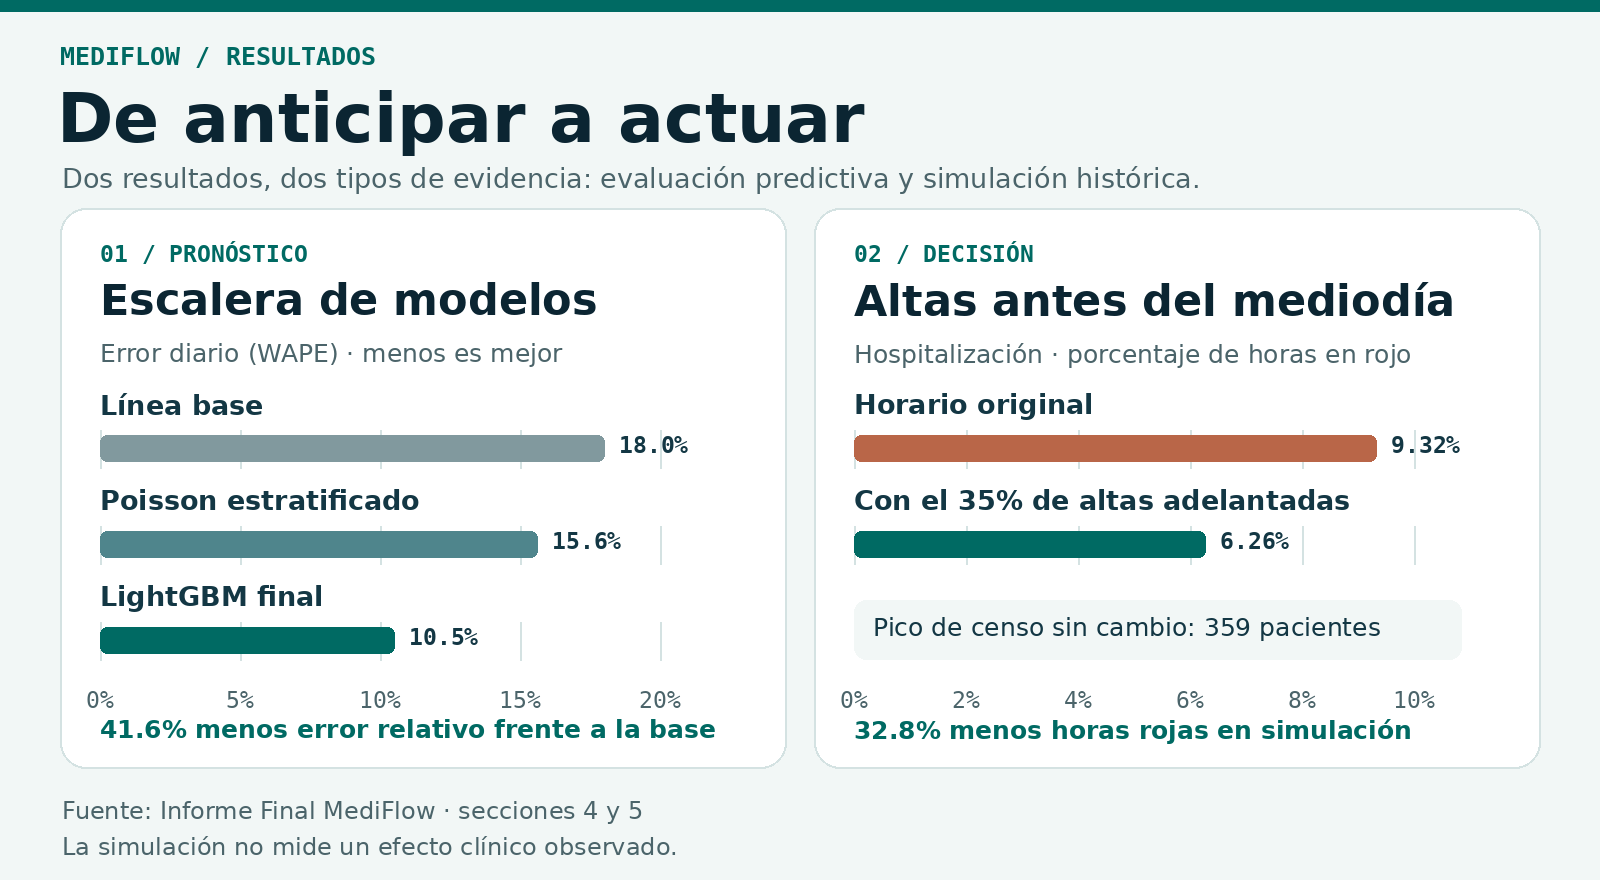
\includegraphics[width=0.92\textwidth]{resumen_escalera_optimizacion.png}
\apanota{Gráfico archivado (\texttt{docs/img/resumen\_escalera\_optimizacion.png}). Los dos paneles representan familias de evidencia independientes: el panel izquierdo corresponde al experimento puntual Poisson en 26 pliegues (WAPE 18,0\,\% $\rightarrow$ 15,6\,\% $\rightarrow$ 10,5\,\%, no al modelo cuantílico web), mientras el panel derecho muestra la simulación histórica determinista de adelanto del 35\,\% de altas en Hospitalización (no un ensayo clínico observado).}
\end{figure}

\subsection{Horizonte extendido a cuatro meses: reporte histórico frente a corrida empaquetada}

Durante el contraste documental contra los artefactos del repositorio se identificó una divergencia relevante entre el reporte Markdown archivado el 3 de noviembre de 2026 \parencite{mediflow2026largoplazo} y la corrida de largo plazo efectivamente empaquetada en el campo \texttt{largo\_plazo} de \texttt{models/modelos\_web\_bundle.joblib} \parencite{mediflow2026bundle} servida por \texttt{GET /api/largo-plazo/\{servicio\}}. Conforme a la decisión editorial aprobada, la Tabla~\ref{tab:largo_plazo_comparado} reporta ambas evidencias por separado sin mezclar sus cifras.

\begin{table}[htbp]
\caption{Desempeño del modelo de largo plazo (120 días, 13 pliegues): reporte archivado frente a bundle servido}
\label{tab:largo_plazo_comparado}
{\singlespacing\small
\begin{tabularx}{\textwidth}{@{}L{0.24\textwidth} Y r r r r r@{}}
\toprule
Fuente y corrida & Servicio & WAPE & $1-\text{WAPE}$ & MAE & Sesgo & Cobertura \\
\midrule
Reporte archivado & Global (sin \texttt{Otros}) & 15,7\,\% & 84,3\,\% & 57,9 & --- & 86,5\,\% \\
(\texttt{2026-11-03}) & Urgencias (\texttt{9203}) & 14,0\,\% & 86,0\,\% & 52,3 & $+20{,}1$ & 85,4\,\% \\
 & Rehabilitación (\texttt{581479}) & 15,5\,\% & 84,5\,\% & 111,7 & $+44{,}2$ & 85,3\,\% \\
 & Tratamiento (\texttt{3045729}) & 64,4\,\% & 35,6\,\% & 9,8 & $+4{,}9$ & 88,7\,\% \\
\midrule
Bundle servido \texttt{v2.0} & Urgencias (\texttt{9203}) & 11,63\,\% & 88,4\,\% & 51,8 & $-15{,}1$ & 87,18\,\% \\
(inspección \texttt{2026-11-19}) & Rehabilitación (\texttt{581479}) & 14,33\,\% & 85,7\,\% & 122,7 & $-2{,}9$ & 83,40\,\% \\
 & Tratamiento (\texttt{3045729}) & 58,12\,\% & 41,9\,\% & 10,1 & $+3{,}9$ & 88,65\,\% \\
\bottomrule
\end{tabularx}}
\apanota{Comparación de dos corridas independientes sobre 13 pliegues solapados (\texttt{2025-03-24} a \texttt{2026-03-19}). La parte superior proviene de \textcite{mediflow2026largoplazo} (donde el WAPE global pasa de 12,2\,\% en el mes 1 a 13,4\,\%, 16,5\,\% y 21,3\,\% en el mes 4, y las proyecciones mensuales agosto--noviembre de 2026 promedian 215,7--221,0 pac./día en Urgencias y 330,5--385,9 en Rehabilitación). La parte inferior proviene de los metadatos inspeccionados en \textcite{mediflow2026bundle} (donde Rehabilitación registra cobertura 77,69\,\% en el mes 1 y 81,79\,\%--87,95\,\% en los meses 2--4, y las proyecciones mensuales promedian 415,6--433,2 pac./día en Urgencias, 661,5--789,6 en Rehabilitación y 15,6--16,1 en Tratamiento). Las proyecciones agosto--noviembre son extrapolaciones desde el corte de julio de 2026 y no corresponden a demanda real observada ni a reentrenamiento con datos de noviembre.}
\end{table}

En el reporte histórico del 3 de noviembre \parencite{mediflow2026largoplazo}, el desempeño agregado cae progresivamente desde 87,8\,\% de exactitud en el mes 1 (WAPE 12,2\,\%) hasta 78,7\,\% en el mes 4 (WAPE 21,3\,\%, ancho medio de banda 424,5 pacientes), y al agregar por semana el servicio de Tratamiento Urgencias alcanza 50,7\,\% de exactitud (WAPE 49,3\,\%). En la corrida empaquetada del bundle \texttt{v2.0}, las tres series muestran menor WAPE en el backtest y proyecciones agosto--noviembre coherentes con los niveles recientes de mediados de 2026 (frente a los promedios notablemente más bajos de la corrida del 3 de noviembre, cuyo origen obedece posiblemente a diferencias previas en el corte o depuración de la serie antes de la actualización de los parquets de entrada), si bien Rehabilitación cae ligeramente por debajo de 80\,\% de cobertura en el primer mes del horizonte (77,69\,\%). El desglose mensual completo de ambas corridas se incluye en el Anexo~B.
